%----------------------------------------------------------------------------------------
%	SECTION X.X
%----------------------------------------------------------------------------------------

\section{Definitions and Examples}

\begin{definition}
    We call the $d$-dimensional vector space  $\R^d$ the  \textbf{Euclidean space}, and it is 
    the set of all vectors (also called points) $(x_1, \dots, x_d)$, where $x_i \in \R$ 
    for  $1 \leq i \leq d$. We define the \textbf{Euclidean norm} to be the function 
    $||\cdot||: \R^d \rightarrow \R$ such that for $x=(x_1, \dots, x_m) \in \R^d$, $||x||=\sqrt{x_1^2+\dots+x_m^2}$; 
    and we define the distance of of two points $x,y \in \R^d$ to be the function 
    $\Delta: \R^d \cross \R^d \rightarrow \R$ such that $\Delta(x,y)=||x-y||$.
\end{definition}

\begin{definition}
    Let $x_1,x_2, \dots, x_m$ be points in $\R^d$. We call a point  $x \in \R^d$, of the form 
   $x=\sum_{i=1}^{m}{\alpha_ix_i}$, with  $\sum{\alpha_i}=1$, a \textbf{convex combination} of $x$. We 
   call the set of all convex combinations of a subset  $A \subseteq \R^d$ the 
   \textbf{convex hull} of $A$, and denote it  $\hat{A}$.
\end{definition}

\begin{definition}
    Let $x,y  \in \R^d$. We call the set  $[x,y]=\{\alpha x+(1-\alpha)y: 0 \leq \alpha \leq 1\}$ of all 
    convex combinations of $x$ and  $y$ an \textbf{interval} with \textbf{endpoints}  $x, y$.

    We call a set  $A \subseteq \R^d$ \textbf{convex} if  whenever $x,y \in A$,  $[x,y] \in A$.
\end{definition}

\begin{example}
   The empty set, regular polyhedra, and open balls in $\R^d$ are all convex. 		
\end{example} 

\begin{figure}
    \centering
    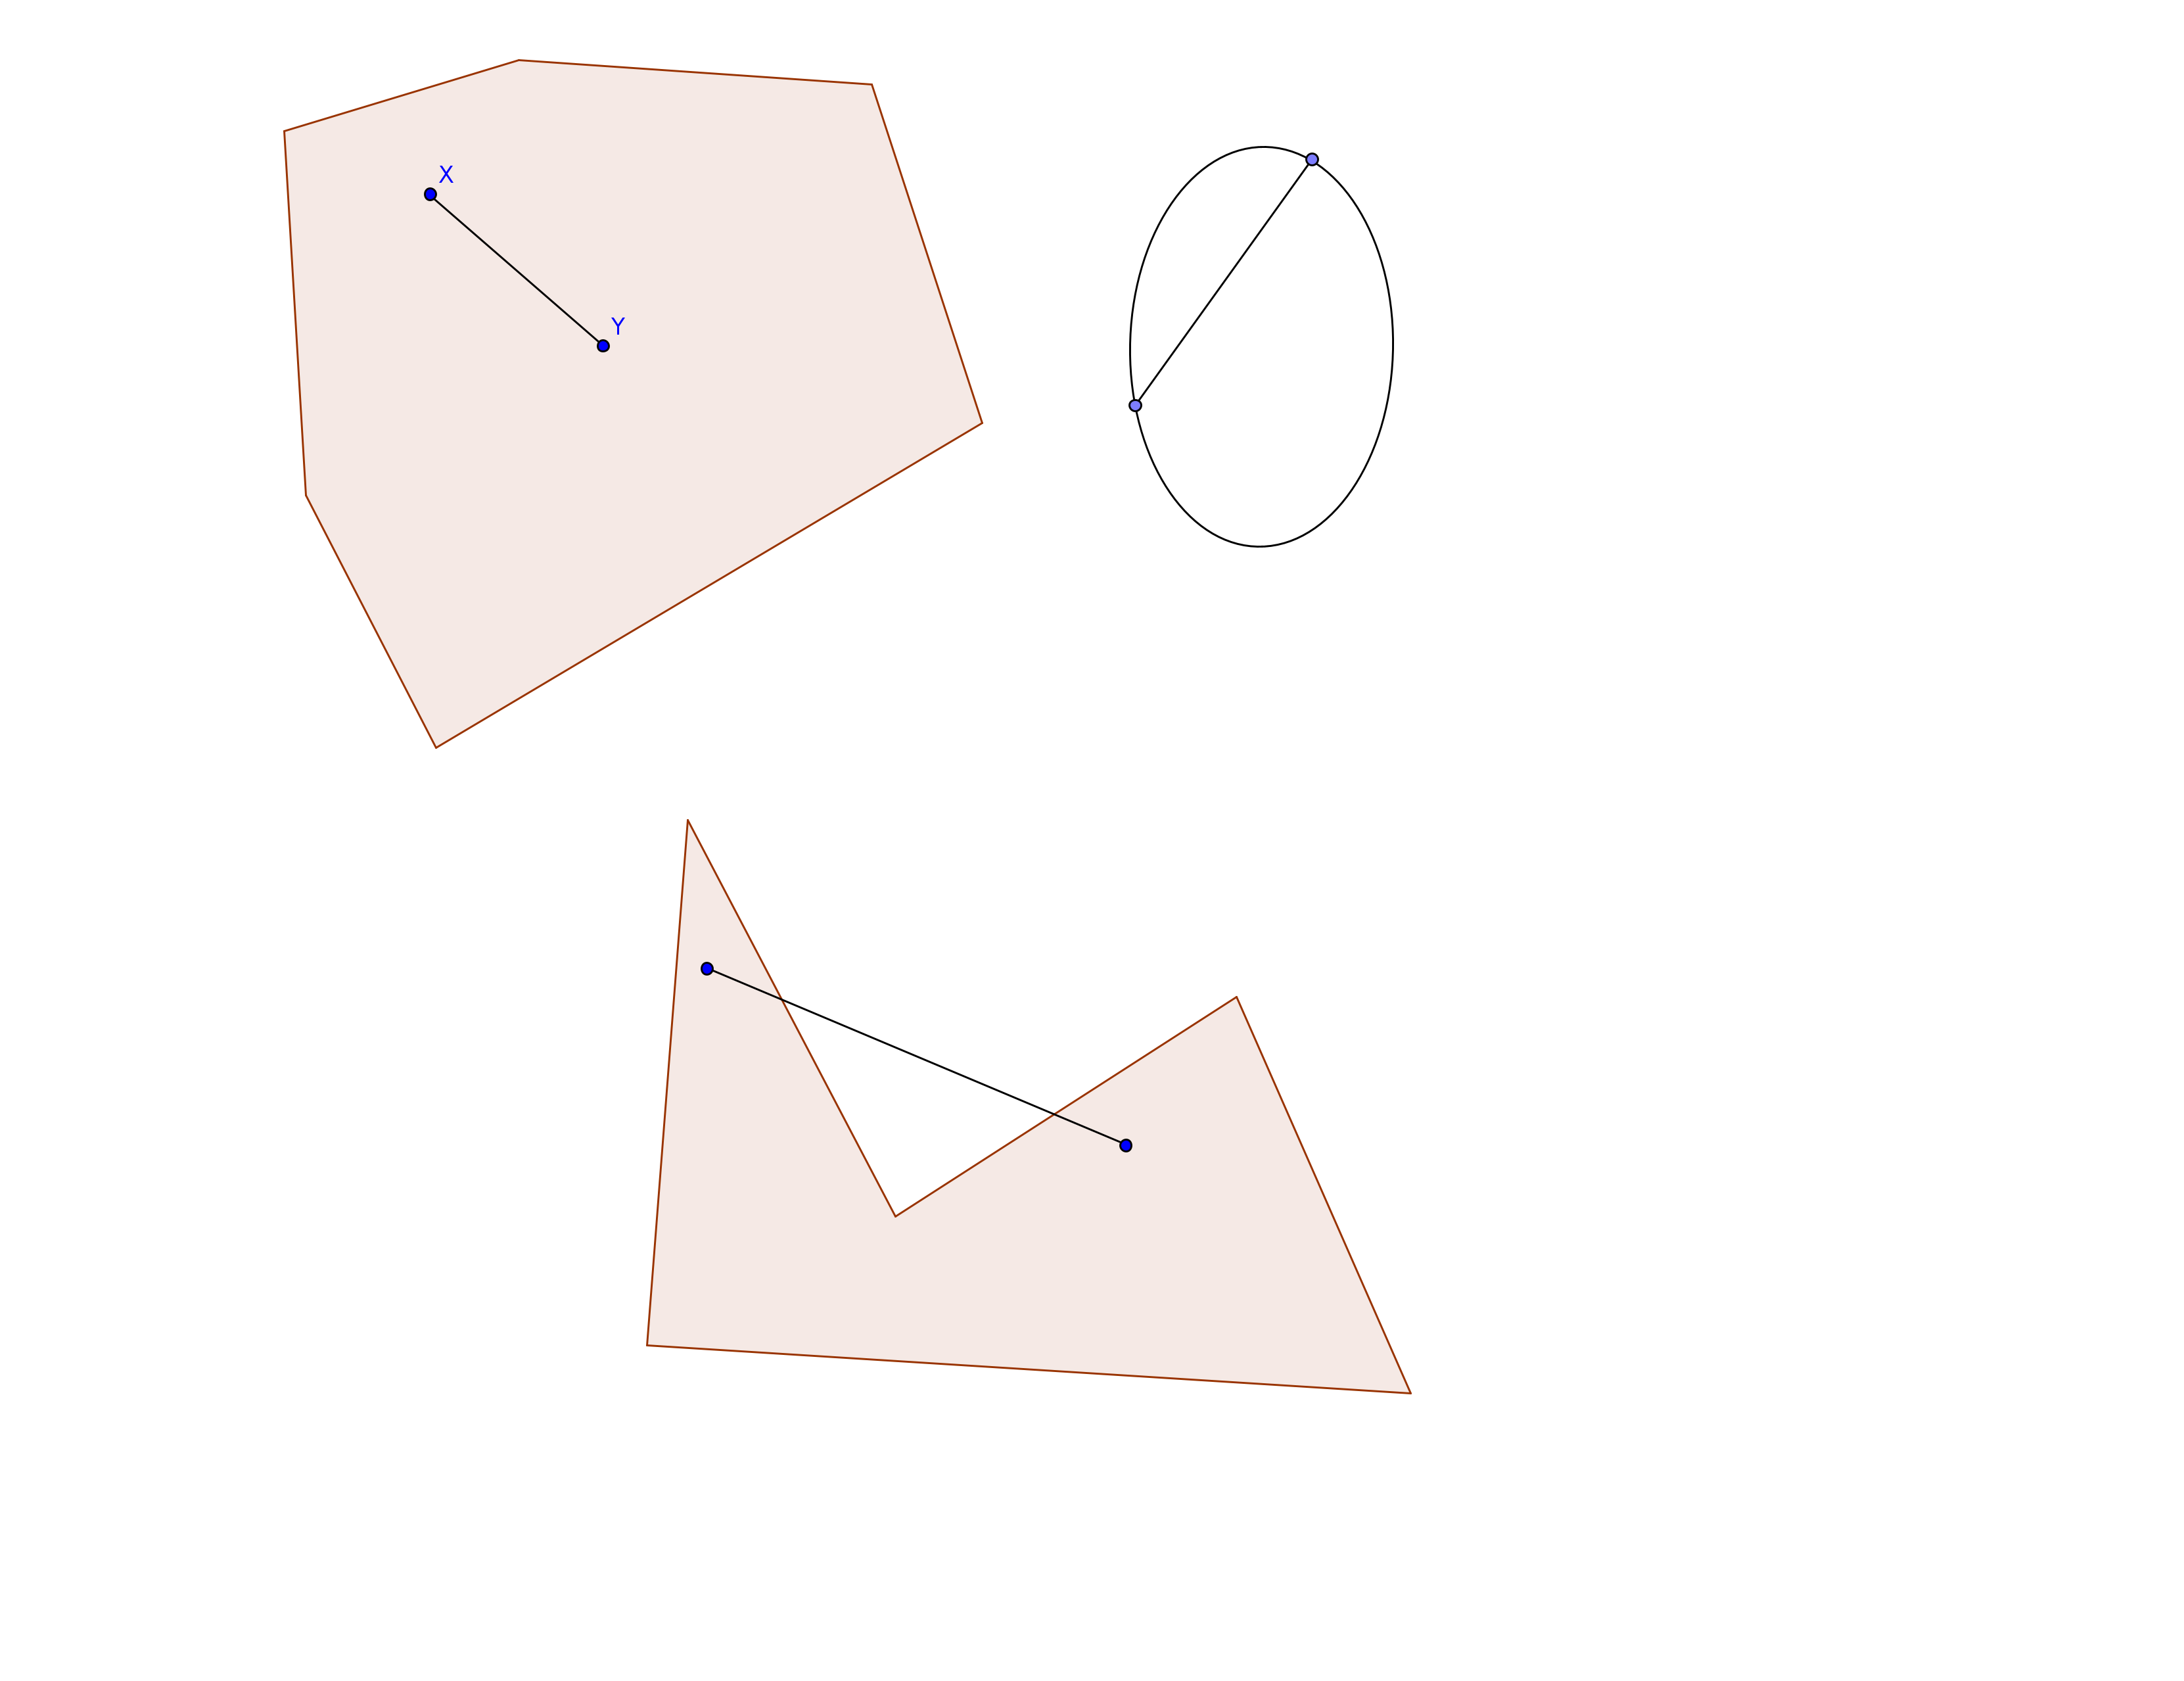
\includegraphics[scale = 0.2]{Figures/convexSets.png}
    \caption{Two convex set, and a non-convex set}.
    \label{fig1.1}
\end{figure}

\begin{lemma}\label{1.1.1}
    The convex hull of a convex set is convex.
\end{lemma}
\begin{proof}
    Let $A \subseteq \R^d$, and let $x,y \in \hat{A}$. Then by definition the set of all convex 
    combinations of $x$ and  $y$ is in  $\hat{A}$, thus  $[x,y] \in \hat{A}$
\end{proof}

\begin{definition}
    Let $c_1, \dots, c_m \in \R^d$ and let $\beta_1, \dots, \beta_m \in \R$; we call the set 
    $A=\{x \in \R^d: \langle{c_i,x}\rangle \leq \beta_i \text{, for } 1 \leq i \leq m\}$ a 
    \textbf{ regular polyhedron}.
\end{definition}

\begin{figure} 
    \centering
    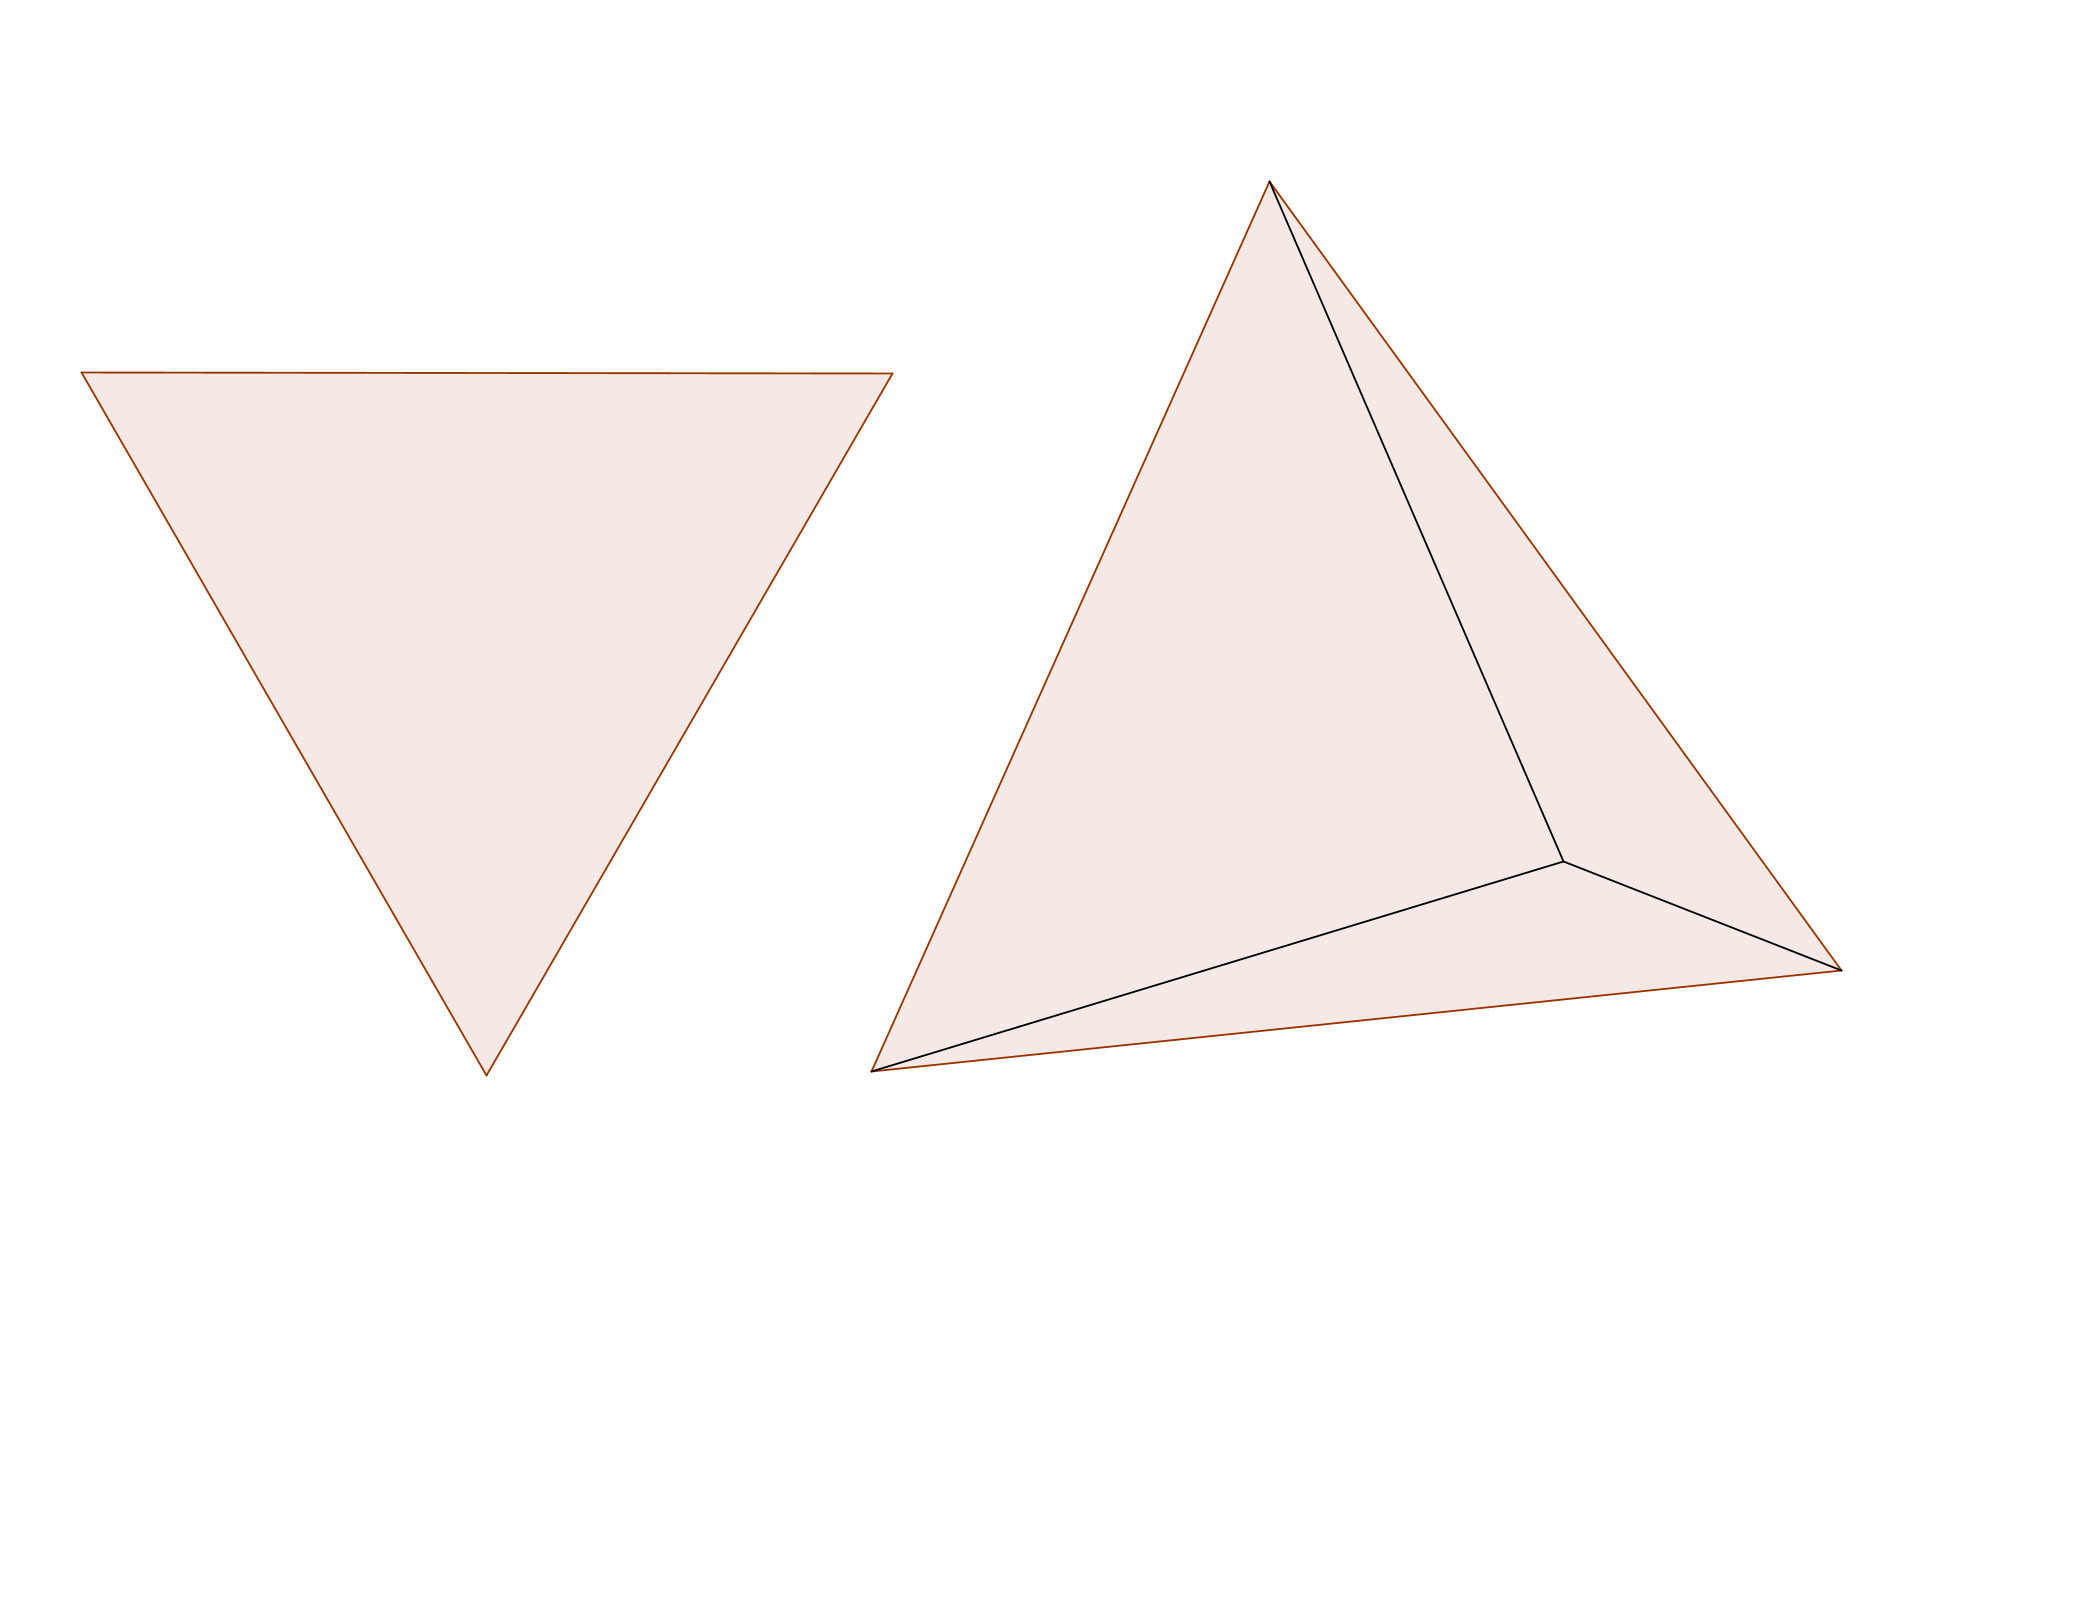
\includegraphics[scale = 0.3]{Figures/regularPolyhedra.png}
    \caption{Regular polyhedra in $\R^2$ and  $\R^3$}
    \fig{fig1.2}
\end{figure}

\begin{lemma}\label{1.1.2}
    Regular polyhedra in $\R^d$ are convex.
\end{lemma}
\begin{proof}
    Let $A \subseteq \R^d$ be a regular polyhedron and let  $x,y \in A$. Then 
    $\langle{c_i,x}\rangle, \langle{c_i,y}\rangle \leq \beta_i$ for $c_i \in \R^d$, $\beta_i \in \R$ 
    for  $1 \leq i \leq m$.Then by the scalar linearity of the innerproduct,  $\langle{c_i, \alpha x+ (1-\alpha)y} \rangle
    \leq \beta_i$. Thus $[x,y] \in $A$.
\end{proof}
